% Generated from the public primitive catalog. Original Atlas drawing; Apache-2.0.
% Target: salsa20; view: detail
\documentclass[border=9pt]{standalone}
% Original Atlas figure theme. Apache-2.0; see the repository LICENSE.
\usepackage[T1]{fontenc}
\usepackage{lmodern}
\usepackage{amsmath,amssymb}
\usepackage{tikz}
\usetikzlibrary{arrows.meta,positioning,calc,fit,backgrounds,decorations.pathreplacing,matrix}
\definecolor{atlasInk}{HTML}{172235}
\definecolor{atlasTeal}{HTML}{0D7B7D}
\definecolor{atlasMuted}{HTML}{637278}
\definecolor{atlasFill}{HTML}{EAF4F2}
\definecolor{atlasLine}{HTML}{B6C8C7}
\tikzset{
  every picture/.style={line width=.65pt,draw=atlasInk,>=Latex},
  every node/.style={text=atlasInk,font=\sffamily\small},
  box/.style={draw,rounded corners=1.5pt,minimum height=.9cm,minimum width=1.6cm,align=center,inner sep=6pt,fill=white},
  accent/.style={box,draw=atlasTeal,fill=atlasFill},
  wire/.style={->,line width=.7pt},
  keywire/.style={wire,draw=atlasTeal,dashed},
  xor/.style={draw,circle,fill=white,inner sep=0pt,minimum size=.38cm},
  add/.style={draw,rectangle,fill=white,inner sep=0pt,minimum size=.38cm},
  note/.style={font=\sffamily\scriptsize,text=atlasMuted,align=center},
  phase/.style={font=\sffamily\small\bfseries,text=atlasTeal},
  group/.style={draw=atlasLine,dashed,rounded corners=2pt,inner sep=8pt}
}
\newcommand{\rotl}{\mathbin{\lll}}
\newcommand{\rotr}{\mathbin{\ggg}}
\newcommand{\kx}{\operatorname{Keccak}\!\text{-}\!f[1600]}

\newcommand{\AtlasKeyBits}{k}
\newcommand{\AtlasKeyWords}{N_k}
\newcommand{\AtlasRounds}{20}
\newcommand{\AtlasPriorRounds}{19}
\newcommand{\AtlasRoundKeys}{21}
\newcommand{\AtlasDoubleRounds}{10}
\newcommand{\AtlasSixRoundGroups}{3.3333333333333335}
\newcommand{\AtlasFLGroups}{2.3333333333333335}
\newcommand{\AtlasRoundStart}{4}
\newcommand{\AtlasBlockBits}{b}
\newcommand{\AtlasOutputBits}{d}
\newcommand{\AtlasStateBits}{512}
\newcommand{\AtlasNonceBits}{64}
\newcommand{\AtlasCounterBits}{64}
\newcommand{\AtlasStreamBlockBits}{512}
\newcommand{\AtlasRate}{r}
\newcommand{\AtlasCapacity}{c}
\newcommand{\AtlasSteps}{N}
\newcommand{\AtlasLastStep}{N-1}
\newcommand{\AtlasWordBits}{64}
\newcommand{\AtlasHashWords}{16}
\newcommand{\AtlasFeedForward}{\boxplus}
\newcommand{\AtlasByteOrder}{big-endian}
\newcommand{\AtlasDomain}{01}
\newif\ifAtlasXof
\AtlasXoffalse
\begin{document}
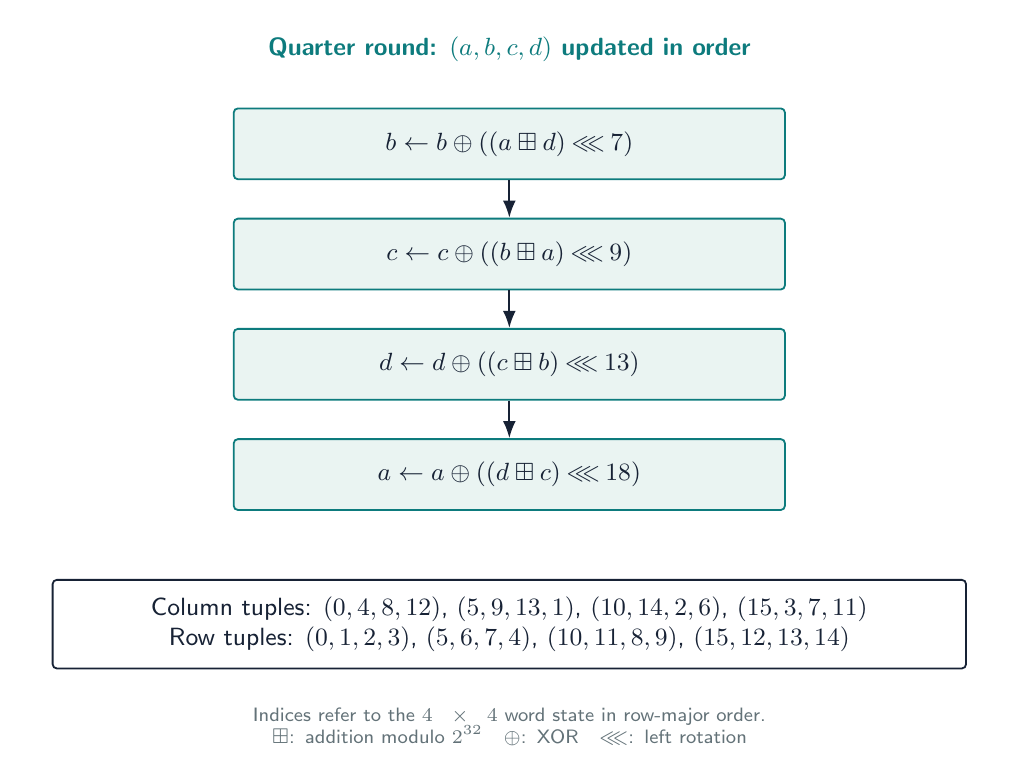
\begin{tikzpicture}
  \node[phase] at (5.8,4.1) {Quarter round: $(a,b,c,d)$ updated in order};
  \node[accent,minimum width=7cm] (q1) at (5.8,2.9) {$b\gets b\oplus((a\boxplus d)\rotl7)$};
  \node[accent,minimum width=7cm] (q2) at (5.8,1.5) {$c\gets c\oplus((b\boxplus a)\rotl9)$};
  \node[accent,minimum width=7cm] (q3) at (5.8,.1) {$d\gets d\oplus((c\boxplus b)\rotl13)$};
  \node[accent,minimum width=7cm] (q4) at (5.8,-1.3) {$a\gets a\oplus((d\boxplus c)\rotl18)$};
  \draw[wire] (q1) -- (q2); \draw[wire] (q2) -- (q3); \draw[wire] (q3) -- (q4);
  \node[box,minimum width=11.6cm] at (5.8,-3.2) {Column tuples: $(0,4,8,12)$, $(5,9,13,1)$, $(10,14,2,6)$, $(15,3,7,11)$\\Row tuples: $(0,1,2,3)$, $(5,6,7,4)$, $(10,11,8,9)$, $(15,12,13,14)$};
  \node[note,text width=12cm] at (5.8,-4.5) {Indices refer to the $4\times4$ word state in row-major order.\\$\boxplus$: addition modulo $2^{32}$\quad $\oplus$: XOR\quad $\rotl$: left rotation};
\end{tikzpicture}

\end{document}
